\section{Multimodal Interaction}

Multimodal interaction is the cornerstone of \textbf{MultiModalMan}. Instead of locking players into a keyboard and mouse loop, the game accepts spoken commands, hand drawn letters captured by a webcam, and classic text input. A Python state manager keeps these channels in sync, while an OpenAI-powered agent interprets free-form utterances and adapts feedback to the current game phase.

\subsection*{Voice Interaction}
\begin{figure}
    \centering
    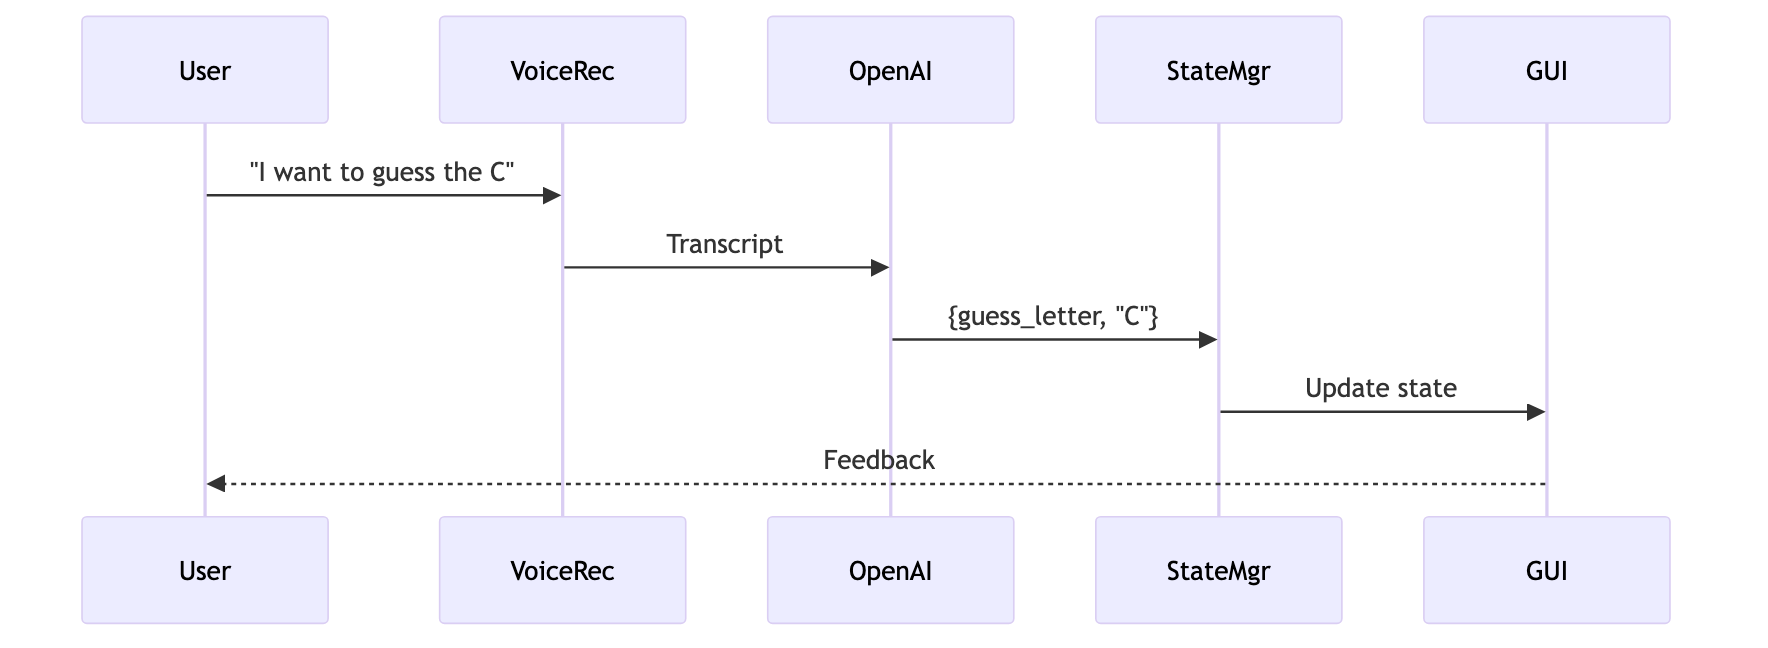
\includegraphics[width=0.55\textwidth]{./images/voice_interaction_flow.png}
    \caption{Activity diagram for the voice interaction component, showing how user speech is processed, transcribed, and routed through the state manager to update the game state.}
    \label{fig:state_machine}
\end{figure}
When the user speaks “start game”, “guess C”, or “exit” for instance the audio stream is transcribed in real time (primary engine: \texttt{speech\_recognition}; fallback: Whisper or the Google Speech API). The recognised text is passed to the state manager, which checks whether the utterance is valid for the current state (setup, guessing, or end of game) and routes it accordingly. Natural phrases such as “how many errors do I have?” are interpreted by the OpenAI agent, which converts them into concrete game actions or informational responses.

\subsection*{Gesture Interaction}
A webcam continuously detects the user’s hand. OpenCV isolates the region of interest, normalises it, and forwards the image to a lightweight CNN trained on finger spelled letters. The predicted character is then forwarded to the state manager, which decides whether to accept, reject, or request clarification always providing on screen feedback so users understand what was recognised.

\subsection*{State Manager}
\begin{figure}
    \centering
    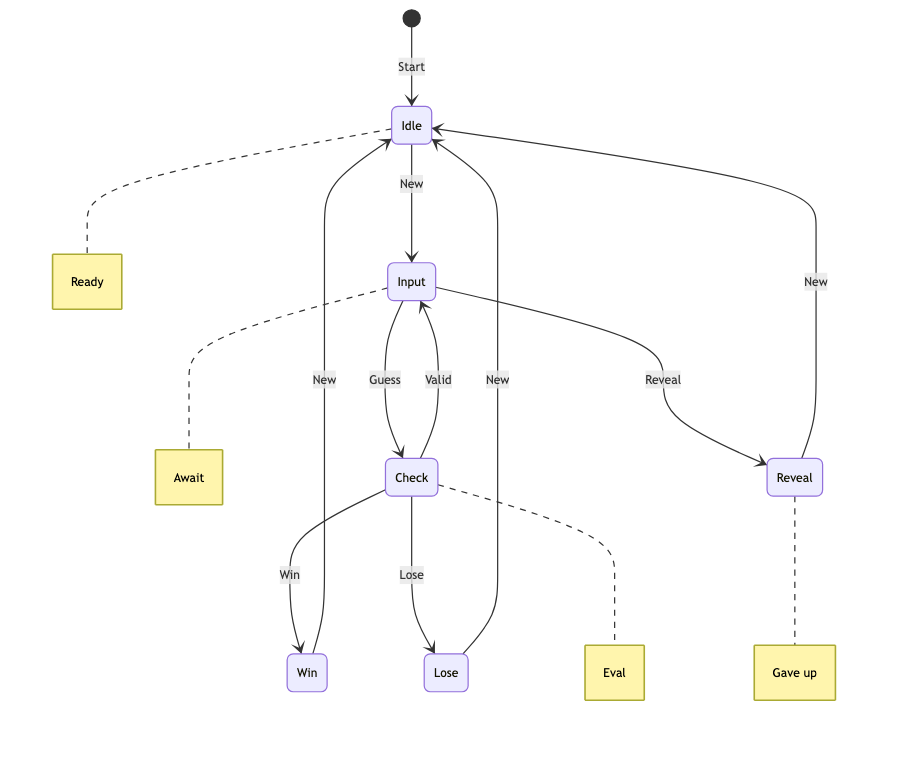
\includegraphics[width=0.5\textwidth]{./images/game_state_manager_state_machine.png}
    \caption{State machine diagram for the \texttt{GameStateManager} class, showing the transitions between different game states based on user inputs and actions.}
    \label{fig:state_machine}
\end{figure}
The \texttt{GameStateManager} class acts as the game’s traffic controller. It tracks a finite set of states (initialisation, waiting for input, verifying, end of game) and exposes two public methods \texttt{handle\_voice\_input()} and \texttt{handle\_gesture()}. Because every modality funnels through this single point, conflicts are resolved centrally: if a gesture and a voice command arrive at the same instant, the manager applies simple time stamping to decide which one to honour first. It also filters commands that make sense only in a given phase (e.g., “new game” is accepted only after a round has finished).

\subsection*{OpenAI Agent}

The agent turns raw language into game intents. It maintains short term context current word, remaining attempts, last hint delivered so that a query like “remind me what I’ve tried” produces a targeted answer.  
Outputs are JSON objects containing an \texttt{action} field (e.g.\ \texttt{"guess\_letter"}) and an optional \texttt{value}.  
This structure lets the state manager treat the agent as just another input device, keeping the architecture loosely coupled.

For security, the OpenAI key is injected via the \texttt{OPENAI\_API\_KEY} environment variable (e.g.\ \texttt{export OPENAI\_API\_KEY=\,$\langle$key$\rangle$} on Unix).

\begin{lstlisting}[style=pystyle,
                   caption={Essential agent scaffold},
                   label={lst:agent}]
agent = Agent(
    name="hangman_game_agent",
    instructions="High-level rules and prompts (truncated for brevity)",
    tools=[
        ("welcome_agent", "Greets and explains rules"),
        ("wordsetter_agent", "Chooses the word"),
        ("letter_guesser_agent", "Processes a letter guess"),
        ("game_restarter_agent", "Starts a new round"),
        ("sync_agent", "Checks active game state"),
    ],
)
\end{lstlisting}
